\subsection{Draft Sequence}
\label{sec:draft-background}

For each capture, the Samsung camera publishes an initial user-visible draft image through the draft sequence, while the post-processing pipeline produces the final image.
When post-processing completes, the final image replaces the draft image if one has been published.
To preserve capture order and limit peak compute and memory demand, the current pipeline executes draft sequences one at a time on a single draft worker.

As post-processing became more resource-intensive, its start was deferred for certain shot modes until the application entered the background to preserve foreground responsiveness.
In these modes, the draft image remains the user-visible result throughout the foreground session, making its visual quality more important.

Yet the original draft sequence saved an image without additional image processing, and advances in post-processing widened the visual gap between draft and final images.
This draft--final visual gap is particularly pronounced in Super-resolution, Night, High-resolution, and Portrait modes, and Figure~\ref{fig:draft-final-gap}(a) and~(c) show an example from Portrait mode.

% Notes: docs/exhibits.md#fig_draft_final_gap
\begin{figure}[!ht]
  \centering
  \setlength{\tabcolsep}{1pt}%
  % All views are the same 1:1 frame (1080 bp source);
  % the zoom box keeps the source region x 162--702, y 695--875 bp from the bottom.
  % TODO: Replace the middle panel and its crop with the actual draft image
  % produced by lightweight multi-frame composition. Both temporarily reuse
  % fig_draft_final_gap_final.jpg; the caption explicitly marks this placeholder.
  \begin{tabular}{@{}ccc@{}}
    \begin{tikzpicture}
      \node[inner sep=0, anchor=south west] (im) at (0,0)
        {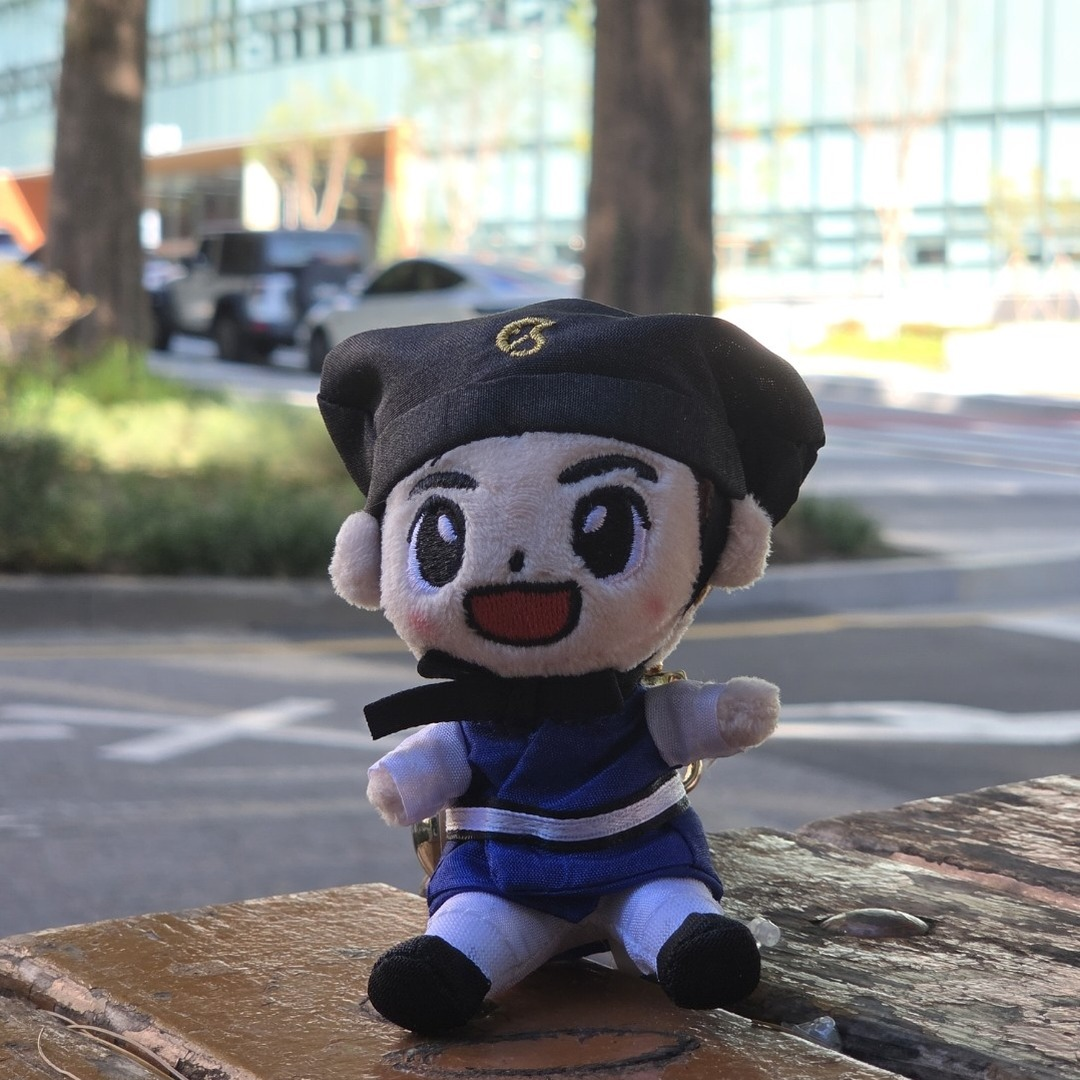
\includegraphics[width=0.325\columnwidth]{figures/fig_draft_final_gap_draft.jpg}};
      \begin{scope}[x={(im.south east)}, y={(im.north west)}]
        \draw[orange, line width=0.8pt] (0.15,0.6435) rectangle (0.65,0.8102);
      \end{scope}
    \end{tikzpicture} &
    \begin{tikzpicture}
      \node[inner sep=0, anchor=south west] (im) at (0,0)
        {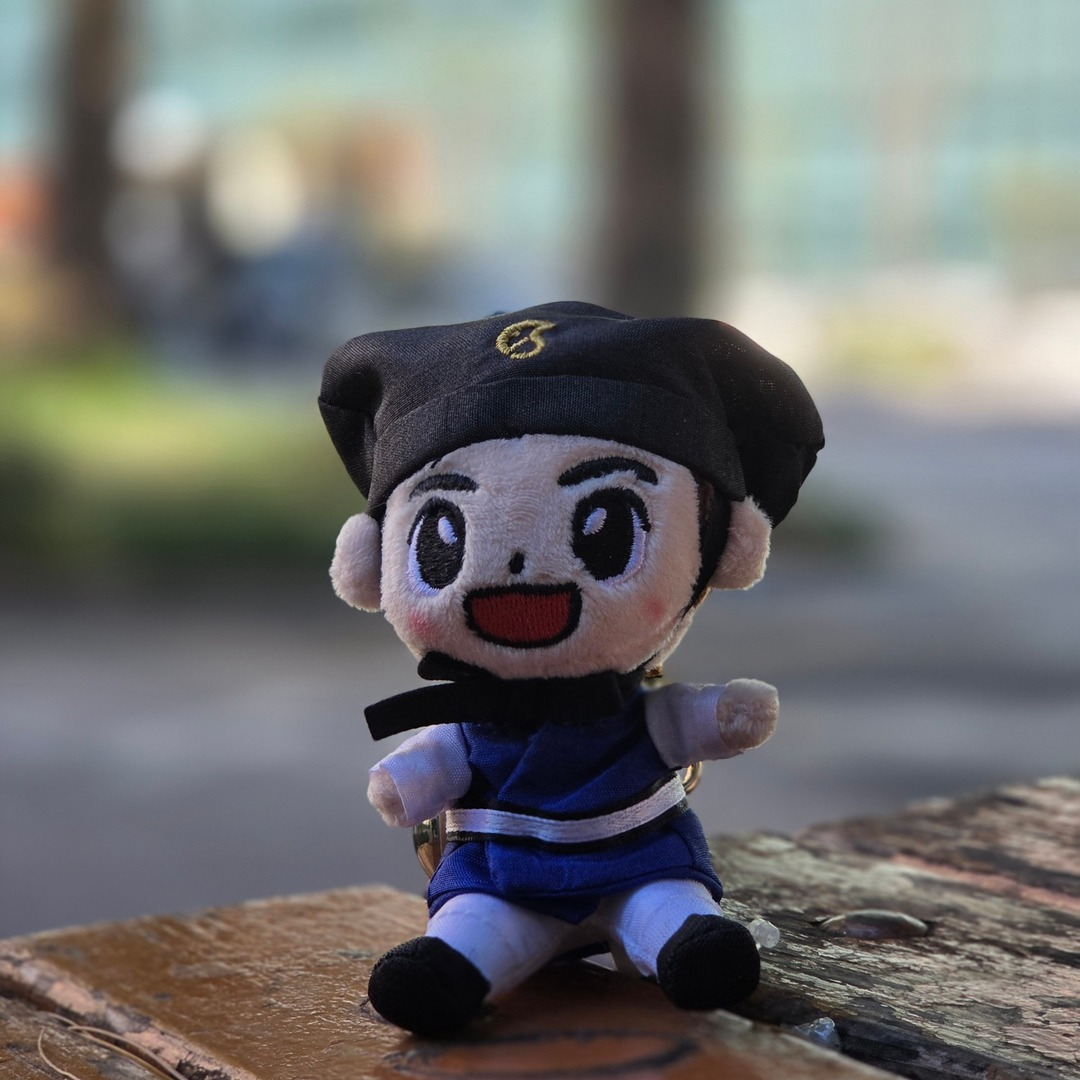
\includegraphics[width=0.325\columnwidth]{figures/fig_draft_final_gap_final.jpg}};
      \begin{scope}[x={(im.south east)}, y={(im.north west)}]
        \draw[orange, line width=0.8pt] (0.15,0.6435) rectangle (0.65,0.8102);
      \end{scope}
    \end{tikzpicture} &
    \begin{tikzpicture}
      \node[inner sep=0, anchor=south west] (im) at (0,0)
        {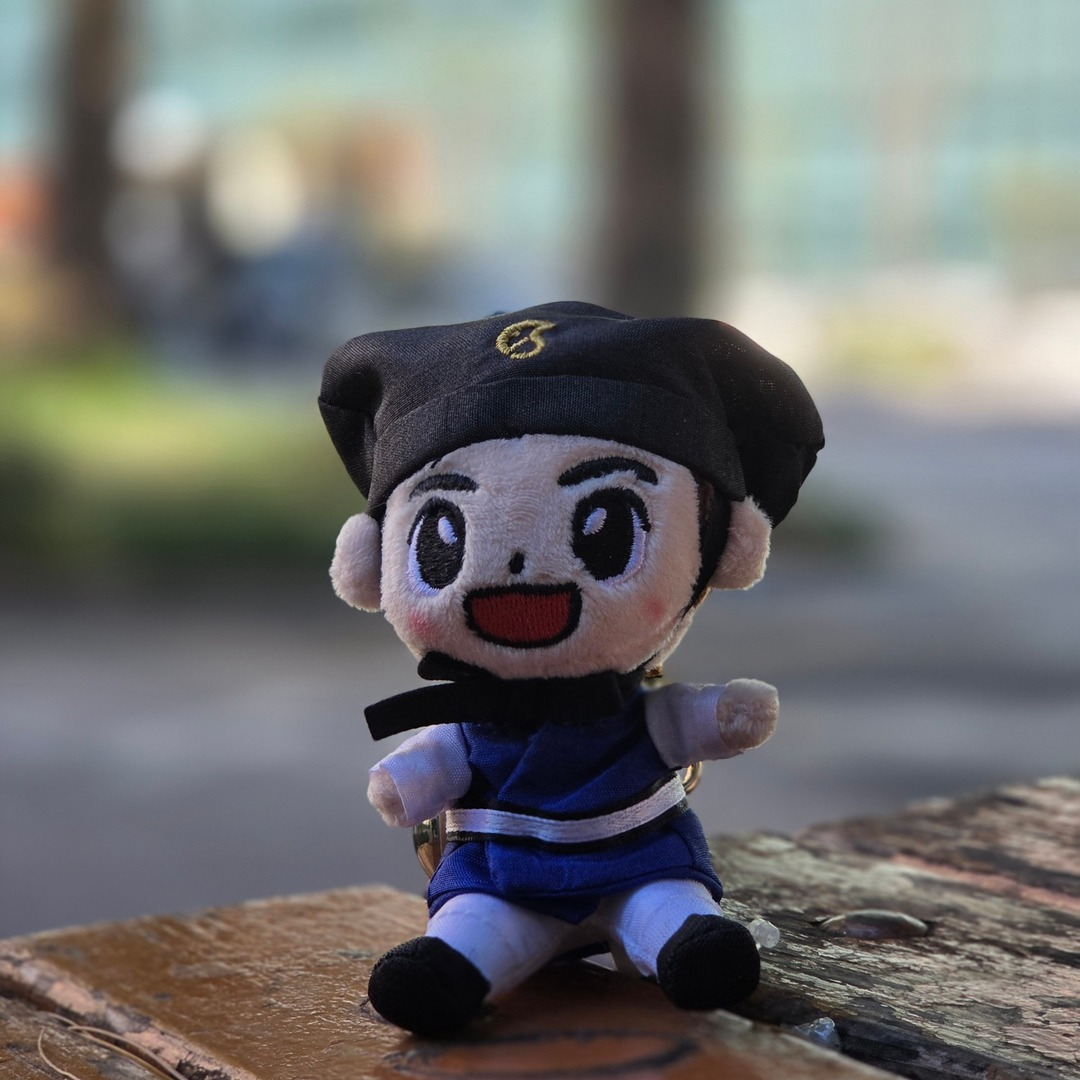
\includegraphics[width=0.325\columnwidth]{figures/fig_draft_final_gap_final.jpg}};
      \begin{scope}[x={(im.south east)}, y={(im.north west)}]
        \draw[orange, line width=0.8pt] (0.15,0.6435) rectangle (0.65,0.8102);
      \end{scope}
    \end{tikzpicture} \tabularnewline[1pt]
    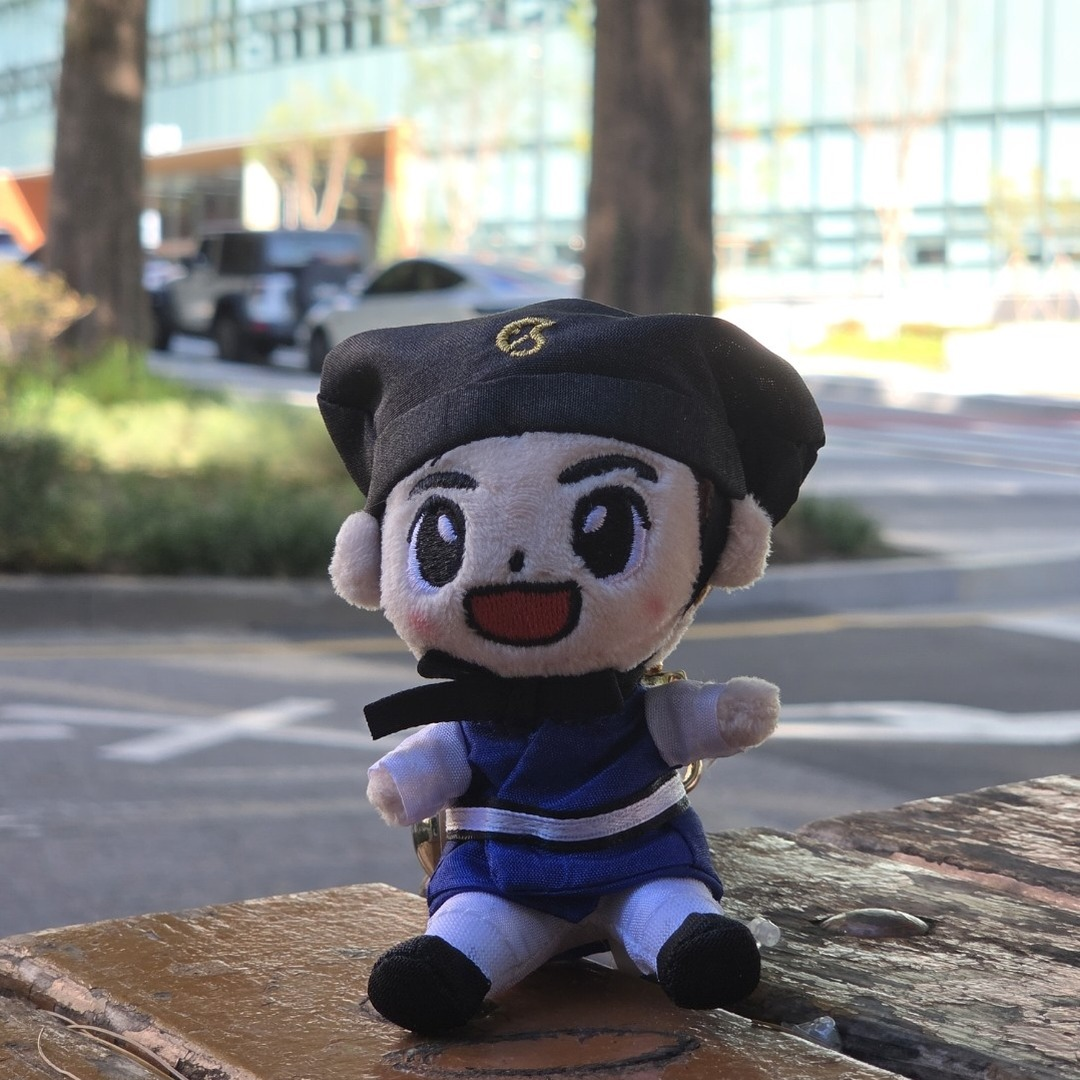
\includegraphics[width=0.325\columnwidth, trim=162 695 378 205, clip]{figures/fig_draft_final_gap_draft.jpg} &
    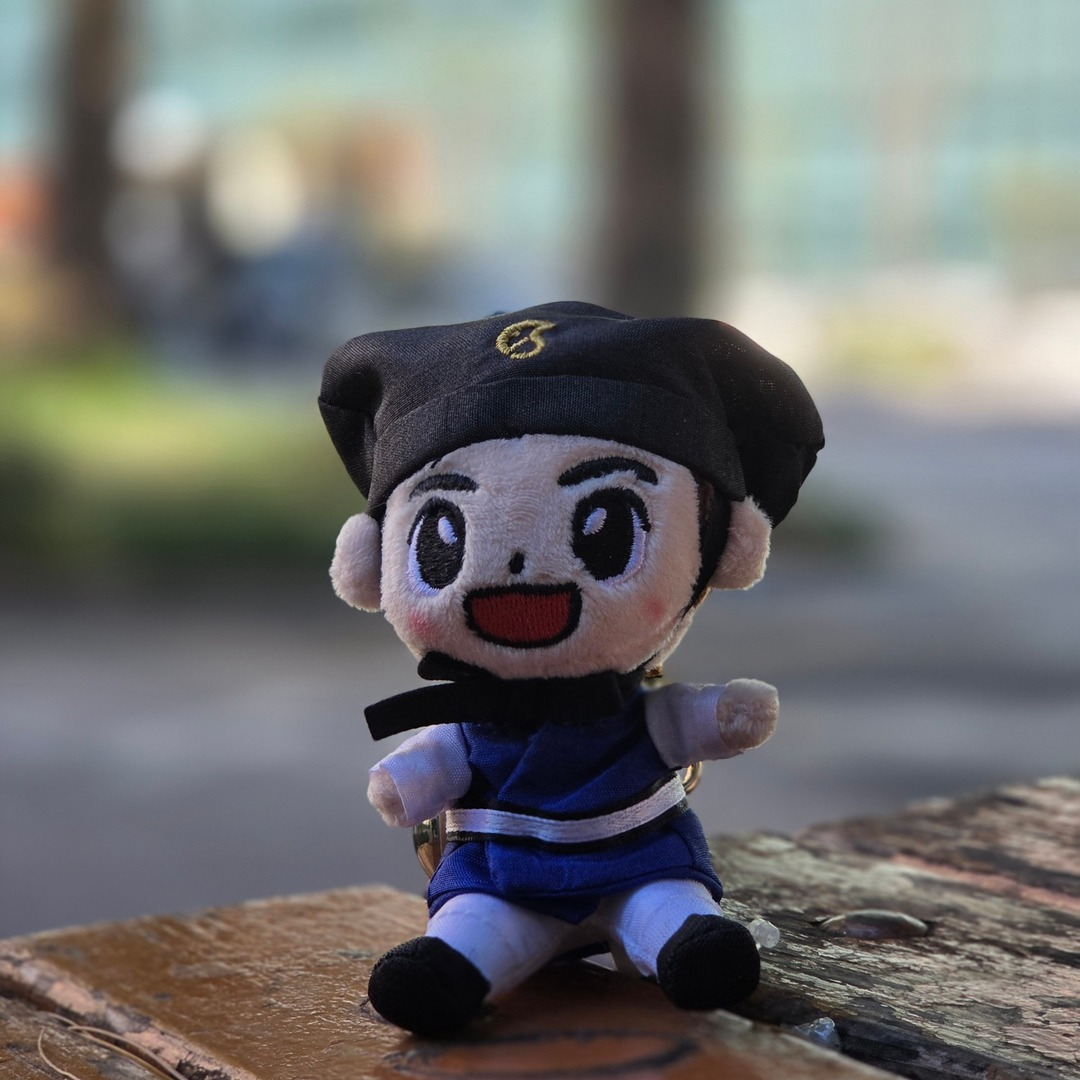
\includegraphics[width=0.325\columnwidth, trim=162 695 378 205, clip]{figures/fig_draft_final_gap_final.jpg} &
    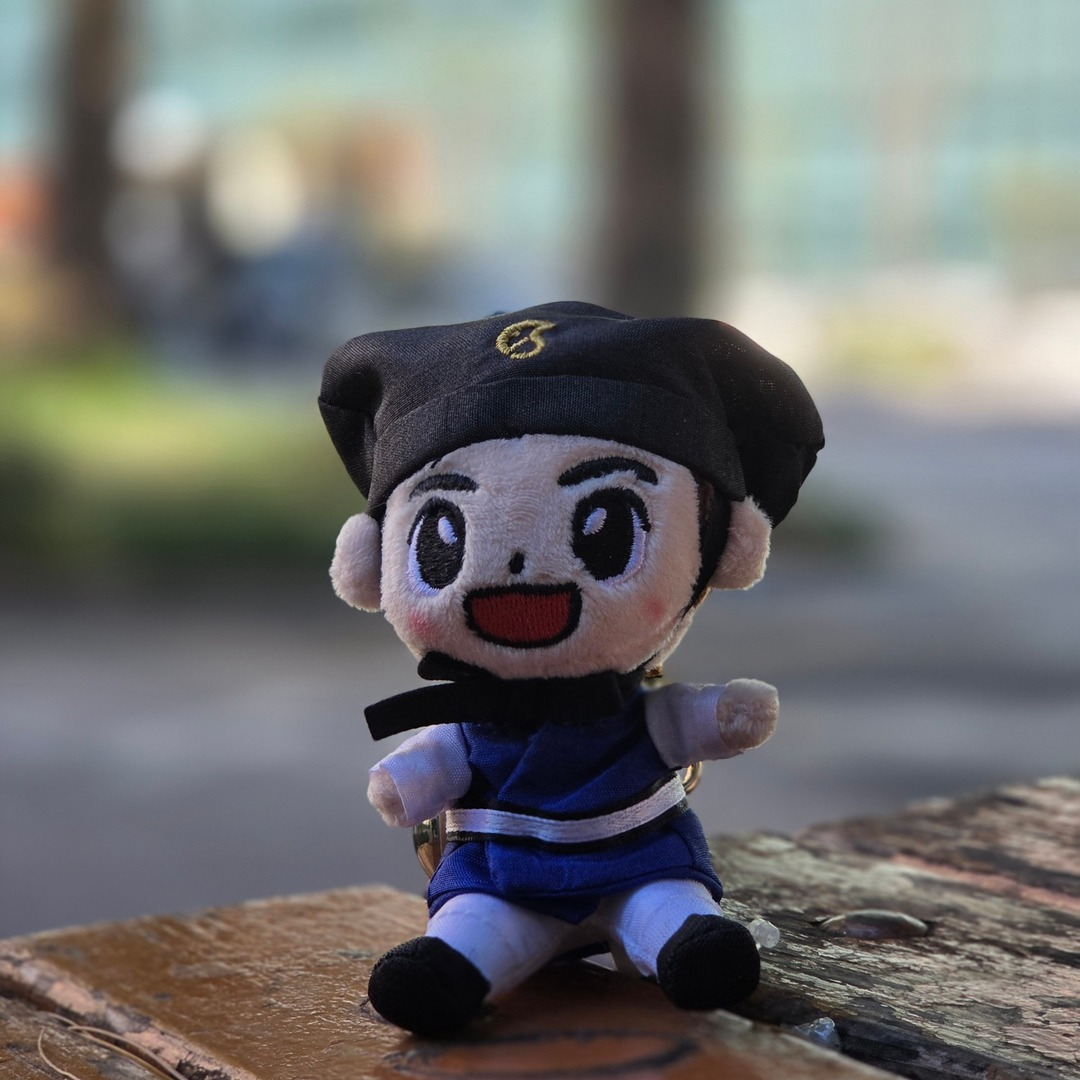
\includegraphics[width=0.325\columnwidth, trim=162 695 378 205, clip]{figures/fig_draft_final_gap_final.jpg}
    \tabularnewline[2pt]
    \parbox[t]{0.325\columnwidth}{\centering\scriptsize (a) Draft image} &
    \makebox[0.325\columnwidth][c]{%
      \parbox[t]{0.41\columnwidth}{\centering\scriptsize
        (b) Draft image with \\lightweight multi-frame composition}} &
    \parbox[t]{0.325\columnwidth}{\centering\scriptsize (c) Final image}
  \end{tabular}
  \caption{Draft--final visual differences in Portrait mode.}
  \label{fig:draft-final-gap}
\end{figure}


\smallskip\noindent\textbf{Extending the draft sequence.}
To reduce this gap, Samsung first added single-frame stages, such as Filter and Watermark, to the draft sequence.
Samsung then implemented lightweight multi-frame composition for Portrait mode to reduce the gap further (Figure~\ref{fig:draft-final-gap}(b)).
However, this additional processing can cause a Capture Timeout, particularly under parallel capture (Section~\ref{sec:parallel-capture}), so the feature has not been deployed on any device model.
